\documentclass[crop=false, class=book]{standalone}

%impostazioni lingua
\usepackage[T1]{fontenc}
\usepackage[utf8]{inputenc}
\usepackage[english,italian]{babel}

\usepackage[dvipsnames]{xcolor}
\usepackage{listings}

\lstdefinelanguage{Kotlin}{
	comment=[l]{//},
	commentstyle={\color{gray}\ttfamily},
	emph={[1]first, firstOrNull, forEach, lazy, map, mapNotNull, println},
	emphstyle={[1]\color{OrangeRed}},
	identifierstyle=\color{black},
	keywords={!in, !is, abstract, actual, annotation, as, as?, break, by, catch, class, companion, const, constructor, continue, crossinline, data, delegate, do, dynamic, else, enum, expect, external, false, field, file, final, finally, for, fun, get, if, import, in, infix, init, inline, inner, interface, internal, is, lateinit, noinline, null, object, open, operator, out, override, package, param, private, property, protected, public, receiveris, reified, return, return@, sealed, set, setparam, super, suspend, tailrec, this, throw, true, try, typealias, typeof, val, var, vararg, when, where, while, it},
	keywordstyle={\color{NavyBlue}\bfseries},
	morecomment=[s]{/*}{*/},
	morestring=[b]",
	morestring=[s]{"""*}{*"""},
	ndkeywords={@Deprecated, @JvmField, @JvmName, @JvmOverloads, @JvmStatic, @JvmSynthetic, Array, Byte, Double, Float, Int, Integer, Iterable, Long, Runnable, Short, String, Any, Unit, Nothing, Config, LightEstimationMode, CameraConfigFilter, CameraConfig, FacingDirection, AugmentedFaceMode, AugmentedFace, TrackingState, RegionType, CloudAnchorMode,AugmentedImageDatabase, BitmapFactory, Session, InstantPlacementMode, File, Uri, RecordingConfig },
	ndkeywordstyle={\color{BurntOrange}\bfseries},
	sensitive=true,
	stringstyle={\color{ForestGreen}\ttfamily},
	emph={[2]FRONT,MESH3D,ENVIRONMENTAL\_HDR,AMBIENT\_INTENSITY, DISABLED,FOREHEAD\_LEFT,FOREHEAD\_RIGHT,NOSE\_TIP, TRACKING, ENABLED, LOCAL\_Y\_UP},
	emphstyle={[2]\color{Purple}\ttfamily},
}

\definecolor{lightgrey}{RGB}{230,237,244}

\lstset{
	basicstyle=\scriptsize\sffamily\color{black},
	backgroundcolor=\color{lightgrey},
	frame=single,
	numbers=left,
	numbersep=5pt,
	numberstyle=\tiny\color{gray},
	showspaces=false,
	showstringspaces=false,
	tabsize=1,
	texcl=true,
	captionpos=b,
	breaklines=true
}




%sistema i margini
\usepackage{geometry}
\geometry{a4paper,top=2.2cm,bottom=2.2cm,left=3cm,right=3cm, heightrounded}

%interlinea 1.5
\usepackage{setspace}
\onehalfspacing

%gestione delle testatine
\usepackage{fancyhdr}
\pagestyle{fancy}
\lhead{}
\chead{}
\rhead{Titolo}
\lfoot{}
\cfoot{\thepage}
\rfoot{}
\renewcommand{\headrulewidth}{0.4pt}

%formattazione titoli paragrafo
\usepackage{titlesec}
\titleformat{\chapter}[block]{\normalfont\huge\bfseries}{\thechapter.}{0.7em}{\huge}

%pacchetti per i riferimenti in bibliografia
\usepackage[autostyle,italian=guillemets]{csquotes}
\usepackage[style=numeric,citestyle=numeric-comp,backend=biber]{biblatex}

%risorsa che contiene la bibliografia
\addbibresource{./../bibliografia.bib}

\usepackage{lipsum}
\usepackage{graphicx}
\usepackage[italian]{varioref}
\usepackage{copyrightbox}



\begin{document}

	\chapter{User Interaction}
	ARCore utilizza la tecnologia \textit{ray casting} per permettere all'utente di posizionare un oggetto nella scena corrente 	in un punto fissato. Quando lo schermo del telefono viene toccato o viene compiuta qualche altra interazione, 					viene proiettato un raggio nella visuale del mondo della fotocamera che può intersecare un preciso punto (costituito da 		due coordinate x,y) o piani geometrici. ARCore permette di ricavare un elenco dei risultati delle intersezioni con la 			geometria della scena rilevata attraverso gli hitTest. Solitamente il primo risultato è quello più significativo 				perchè si riferisce all'intersezione più vicina al dispositivo.\\
	Ogni risultato è costituito da:
	
	\begin{itemize}
		\item[•] Lunghezza in metri dall'origine del raggio.
		\item[•] Posa (posizione e orientamento) del punto toccato.
		\item[•] Istanza Trackable che contiene la geometria 3d che è stata toccata.
	\end{itemize}
	
	\begin{flushleft}
	Questo risultato può essere utilizzato per definire un'ancora che permette di fissare la posizione di 							contenuti virtuali all'interno dello spazio. L'ancora si adatta agli aggiornamenti dell'ambiente circostante e aggiorna gli 	oggetti legati ad essa.\\
	Nella nostra applicazione abbiamo utilizzato l'ancoraggio per due modalità: 
		\begin{itemize}
		\item[•] \emph{Plane Detection}: quando viene premuto lo schermo viene creato un oggetto Anchor sul punto corrispondente dove verrà renderizzato il modello 3D dell'animale selezionato. (Esempio\vref{lst: Definizione Anchor in Plane Detection})
		\item[•] \emph{Augmented Images}: se l'immagine di un pianeta viene riconosciuta viene definito un Anchor nel suo centro nel quale verrà renderizzato il modello 3D del pianeta. (Esempio\vref{lst: Definizione Anchor in Augmented Images})
	\end{itemize}
	\end{flushleft}
	
	\begin{center}
				\begin{minipage}{1.15\textwidth}
					\begin{lstlisting}[caption={Definizione Anchor in Plane Detection}, label={lst: Definizione Anchor in Plane Detection}, language=Kotlin]
					 //Evento che si verifica quando viene toccato un piano
            		 arFragment.setOnTapArPlaneListener { hitResult, plane, motionEvent ->

                	 //Se siamo nella modalità place model
                	 if (!switchButton.isChecked) {

                     arFragment.arSceneView.scene.addChild(AnchorNode(hitResult.createAnchor()).apply {
 
                        // Crea il transformable model e lo aggiunge all'anchor
                        addChild(TransformableNode(arFragment.transformationSystem).apply {

                            setModel()
                            renderable = objRenderable
                            
                            //...
					
				\end{lstlisting}
			\end{minipage}
		\end{center}
	\vspace{0.2cm}
	\begin{center}
			\begin{minipage}{1.1\textwidth}
				\begin{lstlisting}[caption={Definizione Anchor in Augmented Images}, label={lst:Definizione Anchor in Augmented Images}, 	language=Kotlin]
				//Per ogni immagine tracciata  se non è presente il  modello allora viene immediatamente costruito e instanziato
        		for (augmentedImage in augmentedImages) {

            		if (augmentedImage.trackingState == TrackingState.TRACKING) {

                		for (i in 0 until namesobj.size) {

                    		if (augmentedImage.name.contains(namesobj[i]) && !renderobj[i]) {

                        		Toast.makeText(this,""+namesobj[i]+" rilevato",Toast.LENGTH_SHORT).show()

                        		if(namesobj[i]=="systemsolar"){
                            		renderObject(
                                		arFragment,
                                		augmentedImage.createAnchor(augmentedImage.centerPose),
                                		"solar_system"
                            		)
                        		}else {
                            		renderObject(
                                		arFragment,
                                		augmentedImage.createAnchor(augmentedImage.centerPose),
                                		namesobj[i]
                            		)
                        		}	
                        		renderobj[i] = true
                    		}
                		}
            		}
        		}
				\end{lstlisting}
		\end{minipage}
	\end{center}
		
		Esistono quattro tipi di risultati che si possono ottenere in una sessione ARCore:
		\begin{itemize}
		\item[•] \textbf{Profondità}: richiede l'attivazione di depth API nella sessione ARCore ed è usato per posizionare oggetti su superfici arbitrarie (non solo su piani).
		\item[•]\textbf{Aereo}: permette di posizionare un oggetto su superfici piane e utilizza la loro geometria per determinare la profondità e l'orientamento del punto individuato.
		\item[•] \textbf{Punto caratteristico}: permette di disporre oggetti in superfici arbitrarie basandosi su caratteristiche visive attorno al punto sul quale l'utente tocca. 
		\item[•] \textbf{Posizionamento istantaneo}: consente di posizionare un oggetto rapidamente in un piano utilizzando la sua geometria completa attorno nel punto selezionato. 
	\end{itemize}
	
	\begin{figure}
			\centering
			\copyrightbox[0.5]{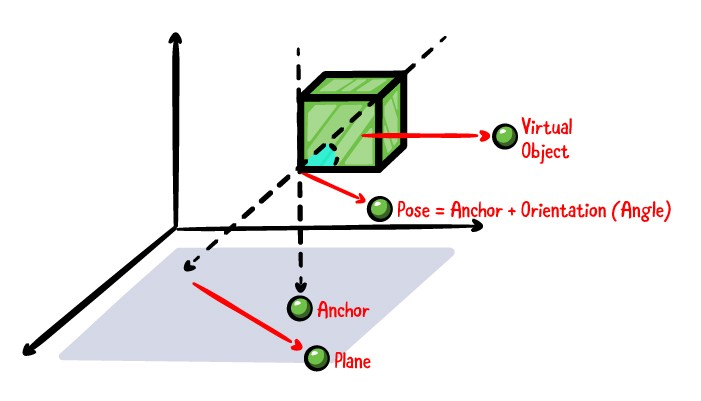
\includegraphics[width=0.8\textwidth]{../../resources/images/UserInteraction/Anchor.jpeg}}%
			{Fonte: \url{https://medium.com/@jaaveeth.developer/arcore-81528569eb2c}}
			\caption{Oggetto virtuale in un piano}
			\label{fig: Oggetto virtuale in un piano}
	\end{figure}
	
	\begin{flushleft}
		Il risultato restituito da hitTest nella modalità \emph{Plane Detection} è di tipo Aereo; il rilevamento di un piano 			consente di disporre un animale in un punto preciso. Questo evento è stato gestito dal metodo 									\textit{setOnTapArPlaneListener} riportato nell'esempio \vref{lst: Definizione Anchor in Plane Detection}.\\
	\end{flushleft}
	
	
			
	
\end{document}